\documentclass[11pt,a4paper]{report}
\usepackage[utf8]{inputenc}
\usepackage{amsmath}
\usepackage{amsfonts}
\usepackage{amssymb}
\usepackage{graphicx}
\usepackage{hyperref}
\usepackage{fullpage}
\begin{document}

\section{NSF Programs}
Below is a list of 3 programs which have been awarded by the NSF and are in the field of cubesats. These are current ongoing programs. 

\subsection{CubeSat: Cubesat investigating Atmospheric Density Response to Extreme driving (CADRE)}
This project is a coordinated science program, whose main instrument is a 3-Unit (3U) CubeSat named Cubesat investigating Atmospheric Density Response to Extreme driving (CADRE). The planned science investigation addresses fundamental issues related to ion-neutral coupling, including neutral wind morphology and dynamics that are key to understanding how the thermosphere reacts to energy input and the role this plays in magnetosphere-ionosphere coupling. Being carried out by Aaron Ridley at UMich currently. \href{http://nsf.gov/awardsearch/showAward?AWD_ID=1042815&HistoricalAwards=false}{The link to the NSF award.}

\subsection{CubeSat: Colorado Student Space Weather Experiment}

The objective of this three-year cross-disciplinary team effort is to build and operate a tiny, so-called CubeSat, spacecraft. The purpose of the 3U Cubesat carrying an energetic particle sensor is to address fundamental space weather science questions relating to the relationship between solar flares, energetic particles, and geomagnetic storms in the near Earth space environment. The particle instrument is the Relativistic Electron and Proton Telescope integrated little experiment (REPTile). REPTile is designed to measure directional differential flux of energetic protons, 10-40 MeV, and electrons, 0.5 to $\textgreater$ 3 MeV.  The specific science objectives for the project are to investigate the relationships between solar energetic particles, flares, and coronal mass ejections, and to characterize the variations of the Earth's radiation belt electrons. Being carried out by Xinlin Li at University of Colorado at Boulder. \href{http://nsf.gov/awardsearch/showAward?AWD_ID=1042815&HistoricalAwards=false}{The link to the NSF award.}

\subsection{Collaborative Research: CubeSat--Composition Variations in the Exosphere, Thermosphere, and Topside Ionosphere (EXOCUBE)}

This project is for a 3U CubeSat mission named EXOCUBE to measure the densities of all significant neutral and ionized species in the upper atmosphere on a global scale. The project will provide the first in-situ global neutral density data in more than 25 years, including the first direct measurements of Hydrogen densities using the mass spectrometer technique. An important science objective for EXOCUBE is to provide observational constraints for physical models of the upper atmosphere. Additionally, the measurements will be used to test and validate newly developed experimental techniques to obtain neutral and ionized composition and densities from radar and optical observations. Being currently done by John Noto at Scientific Solutions Incorporated. \href{http://nsf.gov/awardsearch/showAward?AWD_ID=1042837&HistoricalAwards=false}{The link to the NSF award.}


\section{Small Satellite Conference 2012}
The next topics have been taken from the small satellite conference conducted by KISS. The first few missions listed are all interplanetary missions. Two tables are also given at the end of the section which describe some other missions as well. 

\subsection{Mineral Mapping of Asteroids}
The proposed mission overview is 6U CubeSat launched on a GEO satellite 
or Mars-bound mission as a secondary payload. There is a solar sail to reach near Earth asteroids. The proposed science objectives is to map surface composition of ~3 asteroids at 1-20 m spatial resolution.

Required instrumentation: ~spatial IFOV of 0.5 mrad, spatial sampling 0.5 m -10 m depending on the encounter range, Spectral sampling 10 nm, Imaging Spectrometer, 0.4 – 1.7 $\mu$m. Perhaps extend to 2.5 $\mu$m w/ HOT-BIRD or 
other advanced detector and achievable cooling. 

\subsection{Solar system escape}
The plan is to use use large area/ low mass spacecraft for high speed trajectory with Low perihelion which would Explore interplanetary environment, heliosheath and perhaps heliopause. It is also aimed to Test communications, power, pointing and miniaturized instrument technologies.

Required Instrumentation: Plasma, solar wind, Energetic particles \& cosmic rays, Magnetometer, Cameras to observe sail interaction with environment.

\subsection{Earth-Sun Sunward-of-L1 Solar Monitor}
The aim of this concept is to measure strong Coronal Mass Ejections or other space weather from Sunward-of-L1 position to provide additional warning time to Earth. The science objective is to obtain Plasma and magnetometer readings of solar wind from sunward-of-L1 position to compare with L1 values from ACE or follow-on.

\subsection{Solar Polar Imager CubeSat Constellation}
6 S/C in highly inclined constellation. Out-of-Ecliptic Vertical Orbit, ~0.99 AU. Use solar sail to reach high inclination. The proposed science mission is Dynamo: Helioseismology \& magnetic fields of polar regions. 
Polar view of corona, CMEs, solar radiance, Link high latitude solar wind \& energetic particles to coronal sources. 

The required instrumentation of the 6  satellites are:
\begin{itemize}
\item S/C1: Plasma + Mag Field 
\item S/C2: Energetic Particles + Mag Field 
\item S/C3: Cosmic Rays, 
\item S/C4: Magnetograph/Doppler Imager 
\item S/C5: EUV Imager 
\item S/C6: Coronagraph 
\end{itemize}

\subsection{Radio Quiet Lunar CubeSat}
The aim is to assess radio quiet volume in shielded zone behind the Moon for future 21 cm cosmology missions. The proposed science mission is to find the usable volume behind the Moon for high sensitivity 21 cm cosmology observations which determines utility of lunar surface vs. orbiting missions. 

The other missions provided with no further information are given below. 

\begin{itemize}
\item Sub-L1 Space Weather Monitor 
\item Bright AGN (blazar) monitoring
\item Lunar water mapper
\item QSO survey in NIR
\item Jupiter Aurora (UV) monitor
\item X-ray spectroscopy of ISM, solar wind charge exchange
\end{itemize}

These missions were taken from the presentations given by \href{http://kiss.caltech.edu/workshops/smallsat2012/presentations/murray.pdf}{Stephen Murray} from Space Telescope Science Institute and John Hopkins University and another presentation given by \href{http://kiss.caltech.edu/cosponsored/cubesat2012/presentations/staehle-interplanetary-cubesat-missions.pdf}{Robert Staehle} at JPL. 

The two tables below show some other possible concepts for multiple agents and their required science missions. These were given by Dayton Jones. 


\begin{figure}[!ht]
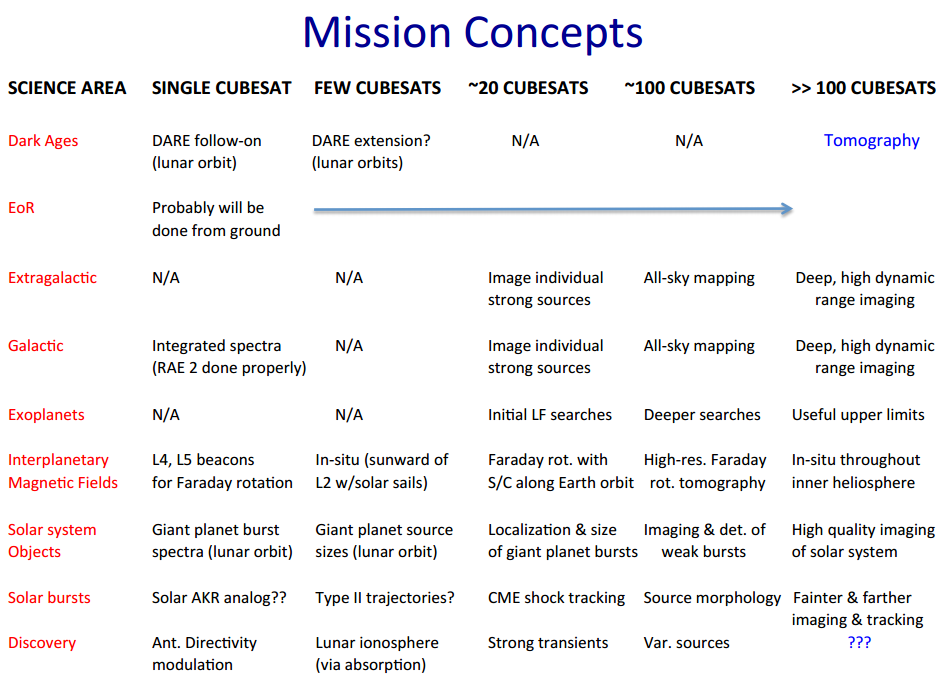
\includegraphics[scale=0.7]{mission_concepts.png}
\caption{Mission concepts for multiple agent systems}
\end{figure}

\begin{figure}[!ht]
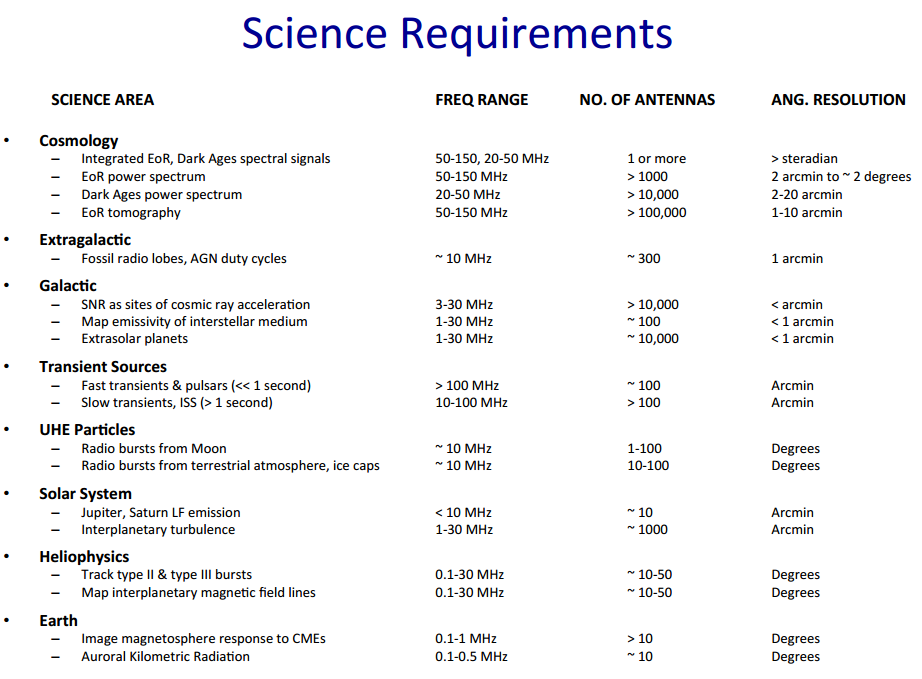
\includegraphics[scale=0.7]{science_req.png}
\caption{Science Requirements for above missions}
\end{figure}

%\bibliographystyle{plain}
%\bibliography{Report}


\end{document}